% =====================================================================
%  c19 —— 原文印刷页 156–164（PDF 第 157–165 页）
%  含：5.2.2 酉性、5.3 一维场论、5.4 二维拓扑场论、5.5 扩展拓扑场论、
%  5.6 三维拓扑场论、5.7 拓扑场论的若干原始文献；第 6 章（6.1–6.4）、
%  第 7 章（7.1、7.1.1）、第 8 章、第 9 章、第 10 章（10.1）开头；
%  插图 Fig. 28–31。
%  说明：原文第 5.3–5.7 小节在稿中大量只存提纲，译文照录其提纲文字。
% =====================================================================

这一简单的观察在物理中非常重要。

当然，态依赖于配边的（拓扑）细节。例如，任何带一个洞的 Riemann 面都定义了从圆周到零的配边，而这样的拓扑有很多。这是量子引力中「Hartle-Hawking」态这一概念的一个原始版本。它也与共形场论中的态／算符对应有关。

\quad b.) 证明：在带定向的配边范畴中，通过交换入边界与出边界（但不改变 $X$ 的定向），同一个流形定义了一个配边 $X^\vee: -Y\to\emptyset$，从而是 $\mathcal{H}(Y^\vee)$ 上的一个线性泛函。

\quad c.) 证明：把这个线性泛函作用于 $\Delta_Y(1)$，会还原出与 $X$ 相联系的 $\mathcal{H}(Y)$ 中的那个原向量。

\quad d.) 证明：若闭流形 $X$ 沿带定向流形 $Y$ 切开而得到 $X_1$ 与 $X_2$，则 $Z(X)$ 可以解释为态 $\psi_{X_1}\in\mathcal{H}(Y)$ 与 $\psi_{X_2}^\vee\in\mathcal{H}(Y^\vee)$ 的一种缩并：
\begin{equation}
  Z(X)=\langle \psi_{X_2}^\vee,\psi_{X_1}\rangle
  \tag{5.24}
  \label{eq:5.24}
\end{equation}
见图~\ref{fig:27}。

\subsubsection{酉性} % 原文: 5.2.2 Unitarity

在酉理论中——当然也在量子力学的公理中——人们要求态空间是复 Hilbert 空间，而配边 $X$ 所对应的 $F(X)$ 应当是酉算符。

现在，一般地，复向量空间 $V$ 上的半双线性形式（sesquilinear form）是一个线性映射 $V\to\bar V^\vee$。因此，在酉理论中改变 $Y$ 的定向相当于对 Hilbert 空间取复共轭：
\begin{equation}
  \mathcal{H}(Y^\vee)\cong\bar{\mathcal{H}}(Y)
  \tag{5.25}
  \label{eq:5.25}
\end{equation}

此外，在物理的酉理论中，$Q_Y$ 上还带有一个正性条件。若 $X: Y_1\to Y_2$ 是配边，那么改变 $X$ 的定向并取对偶，我们便得到配边
\begin{equation}
  \bar X^\vee: Y_2\to Y_1
  \tag{5.26}
  \label{eq:5.26}
\end{equation}
自然地再补上一个条件：
\begin{equation}
  F(\bar X^\vee)=F(X)^\dagger
  \tag{5.27}
  \label{eq:5.27}
\end{equation}
特别地，对闭流形而言，改变流形的定向会使不变量 $Z(X)$ 取复共轭。
% [Tutor Note: (5.26) 的记号 $\bar X^\vee$ 里叠了两个操作，极易读漏其一：上划线是「取复共轭」，即反转 $X$ 的定向；$\vee$ 是「取对偶」，即交换入、出边界。$X:Y_1\to Y_2$ 经这两步叠加才变成 $Y_2\to Y_1$。(5.27) 断言这一复合恰等于 $F(X)$ 的 Hermite 共轭，所以既不能把 $\bar X^\vee$ 只读成「$X$ 的共轭」、也不能只读成「$X$ 的对偶」；核对时请与 (5.25) 对照：那里「变定向 $\Rightarrow$ 复共轭」用的是同一个 $\bar{\ }$，若此处误写为 $\bar X$（不取对偶），(5.27) 两边的边界就不匹配了]

\subsection{一维场论} % 原文: 5.3 One Dimensional Field Theories

考虑带定向的情形。此时 $\mathrm{Bord}^{\mathrm{SO}}_{\langle 0,1\rangle}$ 中的对象是点 $\mathrm{pt}_\pm$（分别带 $+$ 定向与 $-$ 定向）的不交并。

以对称幺半范畴（symmetric monoidal category）$C$ 为值的拓扑场论给出两个对象 $y_\pm=F(\mathrm{pt}_\pm)$，以及如上所述的数据 $\delta$ 与 $q$。一般的对象是 $n_\pm$ 个 $\mathrm{pt}_\pm$ 型点的不交并。这个流形的微分同胚群恰为 $S_{n_+}\times S_{n_-}$，它自然地作用在「态空间」$y_+^{\otimes n_+}\otimes y_-^{\otimes n_-}$ 上。

专门取到 $\mathrm{VECT}_\kappa$，我们便得到一对有限维向量空间 $V_\pm$，连同上面提到的数据：一个非退化配对 $Q: V_+\otimes V_-\to\kappa$，以及「逆」$\Delta: \kappa\to V_+\otimes V_-$。如前所述，这些数据构成 $V_-=V_+^\vee$ 的对偶数据。

这类拓扑场论的一个很好的物理来源，是考虑紧辛流形（compact symplectic manifold）$(M,\omega)$ 的量子化。

一个值得记住的、有用的具体例子是 $M=S^2$，其辛形式为
\begin{equation}
  \omega=\frac{1}{2\hbar}\sin\theta\, d\theta\, d\phi
  \tag{5.28}
  \label{eq:5.28}
\end{equation}
这里 $\hbar$ 是该形式的某个无量纲归一化常数。

在路径积分的 Hamilton 表述中，我们考虑相空间 $M$ 中的路径。我们构造如下形式的路径积分
\begin{equation}
  \int_{\mathcal{P}}[d\gamma]\,\exp[\mathrm{i}S]
  \tag{5.29}
  \label{eq:5.29}
\end{equation}
其中 $\mathcal{P}$ 是 $M$ 中路径构成的空间，$[d\gamma]$ 是由辛形式在路径空间上诱导出的测度，$S$ 是作用量。要使这个表达式有意义，有许多问题需要解决。我们在这里只触及其中几点。

若辛形式 $\omega$ 整体恰当（globally exact），则可写 $\omega=d\lambda$，其中用局部 Darboux 坐标表示
\begin{equation}
  \lambda=\frac{1}{\hbar}pdq
  \tag{5.30}
  \label{eq:5.30}
\end{equation}
一个很好的例子是 $M=T^*X$（$X$ 为某流形）。注意，与这个作用量原理
\begin{equation}
  S[\gamma]=\frac{1}{\hbar}\int_\gamma pdq
  \tag{5.31}
  \label{eq:5.31}
\end{equation}
相联系的 Hamilton 量为零。

但若 $\omega$ 不是恰当的，又当如何？（例如上面 $M=S^2$ 的例子。）让我们先假设 $M$ 是单连通的。此时若 $\gamma$ 是闭路径，我们可以试着这样定义作用量：选取一个圆盘 $\Sigma\subset M$ 使 $\partial\Sigma=\gamma$，然后取
\begin{equation}
  S_\Sigma[\gamma]:=\int_\Sigma \omega
  \tag{5.32}
  \label{eq:5.32}
\end{equation}
若 $\omega$ 恰当，这就回到先前的定义。

现在问题来了：以 $\gamma$ 为边界的圆盘可以不止一个。若 $\Sigma_1,\Sigma_2$ 都以 $\gamma$ 为边界，则 $\Sigma_{12}:=\Sigma_1\cup_\gamma\Sigma_2^\vee$ 是一个 $2$-维闭链，而作用量的不确定性为
\begin{equation}
  S_{\Sigma_1}[\gamma]-S_{\Sigma_2}[\gamma]=\int_{\Sigma_{12}}\omega
  \tag{5.33}
  \label{eq:5.33}
\end{equation}
所以作用量并非良定义。然而，量子路径积分所需的其实只是权重
\begin{equation}
  \exp[\mathrm{i}S]=\exp\Big[\mathrm{i}\int_\Sigma \omega\Big]
  \tag{5.34}
  \label{eq:5.34}
\end{equation}
应当是良定义的。指数化作用量的不确定性是：
\begin{equation}
  \exp[\mathrm{i}S_1]/\exp[\mathrm{i}S_2]=\exp\Big[\mathrm{i}\int_{\Sigma_{12}}\omega\Big]
  \tag{5.35}
  \label{eq:5.35}
\end{equation}
只要 $\omega$ 的周期是 $2\pi$ 的整数倍，左端就等于一，路径积分中也就有了无歧义的权重。请注意，这实际上把「$1/\hbar$」量子化为整数。
% [Tutor Note: 这里「把 $1/\hbar$ 量子化为整数」一句容易读错归一处。关键在 (5.28)：作者一开始就把 $1/\hbar$ 吸收进了辛形式本身（对比 (5.30) 中 $\lambda=pdq/\hbar$），所以 (5.33)–(5.35) 的整性条件是 $\int_{\Sigma_{12}}\omega\in 2\pi\mathbb{Z}$，它约束的是 $\omega$ 里的 $1/\hbar$；若换用「$\omega$ 不含 $1/\hbar$」的约定，同一条件就要改写成对 $\hbar$ 的整性要求。核对 (5.32) 与 (5.31) 是否相容时，务必先确认 $\omega$ 的这一归一化，否则会差一个 $\hbar$ 的幂]

现在，假设 $\gamma$ 不是闭路径。让我们考虑路径空间
\begin{equation}
  \mathcal{P}=\{\gamma:[0,1]\to M\,|\,\gamma(0)=x_0\quad\&\quad\gamma(1)=x_1\}
  \tag{5.36}
  \label{eq:5.36}
\end{equation}
（我们假设 $x_0,x_1$ 位于 $M$ 的同一个道路连通分支中。）在 $\mathcal{P}$ 中选取一条基点路径 $\gamma_0$。那么任何与 $\gamma_0$ 同伦的路径 $\gamma$ 都会使得 $\gamma_0^{-1}*\gamma$ 围出一个圆盘 $\Sigma$。我们随即用这些数据把作用量定义为
\begin{equation}
  S_{\gamma_0,\Sigma}[\gamma]:=\int_\Sigma \omega.
  \tag{5.37}
  \label{eq:5.37}
\end{equation}
对固定的基点路径，只要 $\omega$ 的周期落在 $2\pi\mathbb{Z}$ 中，指数化作用量就与 $\Sigma$ 的选取无关。若把基点路径 $\gamma_0$ 换成同一同伦类中的另一条，作用量只会差一个常数；而实际上，在如上把 $\omega$ 量子化之后，这一选取在指数化作用量中也同样无关紧要。
% [Tutor Note: (5.37) 从「$\gamma$ 与 $\gamma_0$ 同伦」直接跳到「作用量只差常数」，中间被省略的一步是：换基点路径 $\gamma_0\to\gamma_0'$ 时 $\gamma_0'^{-1}*\gamma_0$ 是一条闭道路，于是作用量之差等于 $\omega$ 在该闭道路所围闭链上的周期，而由前面「周期属于 $2\pi\mathbb{Z}$」的假设，指数化之后此差别为 1。也正因这一步只用到了同伦类的信息，(5.37) 对「不与 $\gamma_0$ 同伦的路径」根本没有定义——这正是下一段要处理的问题]

若 $M$ 不是单连通的，就需要额外的考虑：此时即使 $x_0,x_1$ 在 $M$ 的同一道路连通分支中，$\mathcal{P}$ 里仍会有不与 $\gamma_0$ 同处一个道路连通分支的路径。处理这一点的一个办法是在万有覆叠 $\widetilde{M}$ 上工作。最好的做法则是把理论耦合到 $M$ 上的一个平坦联络，以便追踪基本群。
{\small\itshape ［原文标记：EXPLAIN MORE!（要再解释清楚些！）］}
% [原文待办标记，原文 p.158；紧接在「耦合平坦联络以追踪基本群」一句之后，作者自注此处需补充说明]

上面量子化的一个重要特例，是紧单 Lie 群由整权 $\lambda\in\mathfrak{g}^*$ 所定义的余伴随轨道（coadjoint orbit）。这里有一个自然的、整量子化的辛形式，即 Kirillov-Kostant 辛形式；量子化之后给出一个表示，其支配权（dominant weight）向量是 $\lambda$ 的某个适当的 Weyl 旋转。沿着这条思路走下去，可以得到 Borel-Weil-Bott 定理的路径积分解释。在
{\small\itshape ［原文标记：Do it later?（这个以后再做？）］}
% [原文待办标记，原文 p.158；该标记插在句子中间（"In \ensuremath{\clubsuit}...\ensuremath{\clubsuit} the topological field theory"），译文照其位置保留在「在……拓扑场论中」之间]
该拓扑场论中，空间 $V_+$ 是支配权为 $\lambda$ 的表示，空间 $V_-$ 是反支配权为 $-\lambda$ 的共轭表示。对偶数据 $Q$ 是表示与其共轭表示构成单态（singlet）的标准配对，而 $\Delta$ 则是把单态嵌入 $R\otimes R^\vee$ 的映射。
% [Tutor Note: 这一段把 Kirillov-Kostant 形式「可量子化」与「给出不可约表示」两步一笔带过。被省略的是 Borel-Weil-Bott 定理的内容：$\lambda$ 必须是整权（否则该辛形式不是整的、预量子线丛不存在），并且要把 $\lambda$ 用 Weyl 群移到支配 Weyl 腔才对应不可约表示的最高权；非支配的 $\lambda$ 给出的是同一表示的「Weyl 反射」版本。这也是原文为何写 "a suitable Weyl rotation of $\lambda$"。细节可查 Kirillov《Lectures on the Orbit Method》或 Bott 的原始论文]

{\small\itshape ［原文标记：SHOULD ADD MATERIAL ON STOLZ-TEICHNER VIEWPOINT HERE（此处应补入 Stolz-Teichner 观点的材料）］}
% [原文待办标记，原文 p.158；原稿以两行 $*$ 号分隔线上下框住这段全大写文字]

\subsection{二维拓扑场论} % 原文: 5.4 Two-Dimensional Topological Field Theories

需要说明：
\begin{enumerate}
  \item 缝合定理（sewing theorem）与交换 Frobenius 代数；
  \item 如何计算全部振幅；
  \item 半单情形：时空解释；
  \item 开-闭定理（open-closed theorem），以及把边界条件看作某个范畴中的对象；
  \item 半单情形：时空解释；
  \item 如何使理论等变（equivariant）。
\end{enumerate}
以上全部内容：详尽讨论见 GMP2015: [47]。
% 原文此处列表编号为 1.–6.，其中第 1、2 项在印刷页 158，第 3–6 项与末行全大写提示在印刷页 159

\subsection{扩展拓扑场论} % 原文: 5.5 Extended Topological Field Theories

{\small\itshape ［原文标记：CAN ALREADY ILLUSTRATE THE IDEA WITH 2D THEORIES / Follow discussion in [47].（用二维理论就足以说明这一想法。按 [47] 中的讨论进行。）］}
% [原文待办标记，原文 p.159；原稿以两行 $*$ 号分隔线把这两行全大写／普通字体的提示框住]

\subsection{三维拓扑场论} % 原文: 5.6 Three-Dimensional Topological Field Theories

\begin{enumerate}
  \item[5.] 张量范畴（tensor category）。
  \item[6.] 模张量范畴（modular tensor category）。定理：MTC 给出三维酉 TFT。
\end{enumerate}
这一点或许应当放到我们回到三维非阿贝尔 Chern-Simons 之后再讲？
% 原文此处两项的编号沿用前一小节的列表，分别为 5. 与 6.（第 6 项缩进一级）

\subsection{拓扑场论的若干原始文献} % 原文: 5.7 Some Source Material For Topological Field Theories

关于拓扑场论有极其庞大的文献。早期的一篇关键论文是

\qquad 1.\ M.F. Atiyah, ``Topological quantum field theories.'' Inst. Hautes Etudes Sci. Publ. Math. No. 68 (1988), 175-186 (1989).

这篇论文受到 Witten 的工作以及 Graeme Segal 对共形场论的公理化表述的启发，后者现在可见于：

\qquad 2.\ G. Segal, ``The Definition Of Conformal Field Theory,'' 载于 \emph{Topology, Geometry and Quantum Field Theory: Proceedings of the 2002 Oxford Symposium in Honour of the 60th Birthday of Graeme Segal}。

若想要一份更多从物理学家视角写成的导引，请看

\qquad D. Birmingham, M. Blau, M. Rakowski,m and G. Thompson, ``Topological Field Theory,'' Phys.\ Rept.\ 209 (1991) 129-340

我们还参考了讲义

\qquad 3.\ Segal, Stanford notes, \texttt{http://www.cgtp.duke.edu/ITP99/segal/}

以及这篇综述性文章：

\qquad 4.\ G. Segal and G. Moore, ``D-branes and K-theory in 2D topological field theory'' hep-th/0609042。另见 P. Aspinwall 等，\emph{Mirror Symmetry II}, Clay Mathematics Institute Monograph 一书的第 2 章。

关于拓扑场论的一般情形，极为细致审慎的讨论见

\qquad 5.\ V.G. Turaev, \emph{Quantum Invariants Of Knots And 3-Manifolds}, De Gruyter, 2nd edition 2010.

$d=3$ 的 TQFT 与模张量范畴这一特例，最早得到详细描述是在

\qquad G. Moore and N. Seiberg, ``Lectures on RCFT,'' 载于 \emph{Superstrings '89}, World Scientific, pp.\ 1-129.

其后的专著

\qquad Bakalov and Kirillov

给出了更细致的处理。

我们用到了 Dan Freed 那份非常好的讲义中的一些材料：

\qquad 10.\ D. Freed, ``Bordism Old And New,'' \texttt{https://www.ma.utexas.edu/users/dafr/M392C-2012/index.html}

关于高阶范畴论与局域性的近期进展，请看

\qquad 11.\ A. Kapustin, ``Topological Field Theory, Higher Categories, and Their Applications,'' arXiv:1004.2307 [math.QA]

\qquad 12.\ J. Lurie, ``On the classification of topological field theories,'' arXiv:0905.0465 [math.AT]

\qquad 13.\ D. Freed, ``The cobordism hypothesis'' BAMS

\qquad 14.\ D. Freed, ``Remarks On Chern-Simons Theory,'' Bull.\ AMS, 46 (2009), pp.\ 221-254
% 原文此处的文献编号从 5. 直接跳到 10.（作者原稿的编号不连续），译文照原编号保留

\section{用 RCFT 计算非阿贝尔 Chern-Simons 关联函数} % 原文: 6. Computing Nonabelian Chern-Simons Correlators Using RCFT

\begin{keytakeaways}
  \item 核心事实：在手征代数的不可约表示所对应的典范基下写出的模变换 $S$ 矩阵，等于 $S^3$ 中两条相互链接的圆上、分别带有对应表示的线缺陷时路径积分的值。原稿在图~\ref{fig:10} 中「从实验上」观察到了这一点，本节说明它实际上相当普遍。
  \item 论证只依赖两条关键事实：(i) 两个 $D^2\times S^1$ 柄体沿边界粘合，若按 $D^2$ 粘成球面的方式粘，得到 $S^2\times S^1$；若用交换两个圆周期的 $S$ 变换粘，得到 $S^3$。(ii) 沿柄体核心插入线缺陷会在 $\mathcal{H}(T^2)$ 中产生态。
  \item 粘合前必须对两个态之一作用 $S$；配合 $\mathcal{H}(T^2)$ 上使 $\chi_i$ 正交归一的双线性形式，即可读出 $S$ 矩阵与链接圆上路径积分的相等关系。
  \item 对 Verlinde 公式，原稿只给了一条「奥林匹亚式」的捷径：按 Moore-Seiberg《Lectures on RCFT》习题 7.13 走一遍。
\end{keytakeaways}

\subsection{编织矩阵与融合矩阵的三维解释} % 原文: 6.1 3D Interpretation Of Braiding And Fusing Matrices
% 原文此小节只有标题，没有正文（原稿在此仅留标题，内容显然尚待补写）

\subsection{手术操作} % 原文: 6.2 Surgery Manipulations

\subsubsection*{模 $S$ 矩阵的三维解释}
% 原文此行是一个无编号的下划线小标题（位于 6.2 之下、6.3 之前）；因其无编号，用带星号的标题复刻，不参与自动编号

我们在图~\ref{fig:10} 中从实验上观察到：模变换 $S$ 矩阵——在以对应于手征代数不可约表示的典范基写出时——等于 $S^3$ 中带有相应表示的线缺陷的两条链接圆上路径积分的值。事实上，这个关系相当普遍，我们现在就来解释。

我们需要两条关键事实：

\begin{enumerate}
  \item 取两份柄体（handlebody）$D^2\times S^1$。其边界是 $S^1\times S^1$，其中第一个 $S^1$ 因子是 $D^2$ 的边界。若把这两个柄体粘在一起，使两份 $D^2$ 粘成一个球面，则所得的闭 $3$-流形是 $S^2\times S^1$。另一方面，若用一个交换两个圆周期的 $S$ 变换来粘这两个 $T^2$ 因子，则所得的 $3$-流形是 $S^3$。看清这一点有一个相当快捷的办法：注意到所得的 $3$-流形是单连通的，因为环面中的 $a,b$ 两个圈可以在其中一个或另一个柄体里连续收缩为一点。然后引用 Poincaré 猜想即可。一个更初等的证明是……
  {\small\itshape ［原文标记：GIVE A PROOF THAT DOES NOT RELY ON POINCARE（给出一个不依赖 Poincaré 猜想的证明）］}
  % [原文待办标记，原文 p.160；紧接在「一个更初等的证明是……」之后，作者自注此处需要一个不依赖 Poincaré 猜想的证明]

  \item 现在考虑沿上述两个柄体各自的核心插入线缺陷的路径积分，一个对应表示 $i$、一个对应表示 $j$。它们在该 $\mathcal{H}(T^2)$ 中产生相应的态 $\chi_i,\chi_j$。这个空间上有一个双线性形式，使得这些态在其中正交归一。另一方面，当我们用模变换来粘合边界时，必须在粘合前对两个态之一作用 $S$。一般结果便随之得到。
  {\small\itshape ［原文标记：NEED TO EXPLAIN!!（此处需要解释！！）］}
  % [原文待办标记，原文 p.160；针对「粘合前须对两态之一作用 $S$」这一步]
\end{enumerate}

{\small\itshape ［原文标记：EXPLAIN THIS BETTER.（这一点要解释得更好。）］}
% [原文待办标记，原文 p.161；位于「一般结果便随之得到」之后]

Verlinde 公式的奥林匹亚式证明：按 Moore-Seiberg《Lectures on RCFT》习题 7.13 做。
% [Tutor Note: 这里的「奥林匹亚式证明」指一跳到底、只留关键动作的证明。习题 7.13 的实际内容是用 (i) 中两种粘合方式给出的态的内积、以及 (ii) 中 $S$ 对其中一个态的作用，把 Verlinde 公式 $N_{ij}^{\ \ k}=\sum_n S_{in}S_{jn}S_{kn}^*/S_{0n}$ 化成一次矩阵乘法；缺的中间步骤是「粘贴两次得到 $S^2$ 的矩阵元关系」。若手头没有 Moore-Seiberg 讲义，可对照 Bakalov-Kirillov 第 3 章中同一结论的推导]

\subsection{Jones 多项式与 WRT 不变量} % 原文: 6.3 The Jones polynomial and WRT Invariants

\begin{enumerate}
  \item 纽结不变量与 Reidemeister 移动；
  \item skein 关系；
  \item Jones 多项式；
  \item 推广：按 Witten 的着色 Jones 多项式；
  \item 路径积分：WRT 不变量；
  \item 用编织、融合与 $S$ 矩阵的数据进行计算。
\end{enumerate}

\subsection{超越纽结多项式：范畴化与纽结同调的想法} % 原文: 6.4 Beyond knot polynomials: The idea of categorification and Knot homology.

\section{有限群 Chern-Simons 理论} % 原文: 7. Finite Group Chern-Simons Theory

\begin{keytakeaways}
  \item 三维 Chern-Simons 理论对\emph{任意}紧 Lie 群都可以定义（前文讨论的多是单连通或单的情形，这里强调的是「任意」）；一般紧 Lie 群的结构见附录 J.1。
  \item 当规范群取有限群 $G$ 时，理论由群上同调（group cohomology）刻画，其分类空间 $BG$ 的上同调给出理论的数据。
  \item 「能级」（level）在这一情形下的自然归宿是 $H^4(BG;\mathbb{Z})$；相应文献为 Dijkgraaf-Witten 与 Freed（原文此处拼作 ``Dijgraaf''）。
\end{keytakeaways}

\subsection{一般紧群 $G$} % 原文: 7.1 The General Compact Group G

三维 Chern-Simons 理论可以对任意紧 Lie 群定义。关于一般紧 Lie 群长什么样，可参见附录 J.1。

\subsubsection{规范群为有限群时的 Chern-Simons 理论} % 原文: 7.1.1 Chern-Simons Theory When The Gauge Group Is A Finite Group

群上同调。

群上同调与 $BG$。

能级的自然归宿是 $H^4(BG;\mathbb{Z})$。

引用：Dijgraaf-Witten。Freed。
% 以上四行在原稿中即为提纲式短语（其中 "Dijgraaf" 系原稿拼法，通常拼作 Dijkgraaf），译文照录

\section{$p$-形式推广与微分上同调} % 原文: 8. p-form Generalizations And Differential Cohomology

\begin{keytakeaways}
  \item 本节只留下提纲：微分上同调（differential cohomology）的回顾，按 FK 讲义中的相应章节进行。
  \item 需要强调的要点是：阿贝尔 Chern-Simons 作用量不过是 Cheeger-Simons 的「相乘并积分」双线性形式的一次二次加细（quadratic refinement）。
  \item 本节在本片段中只有这两条提纲、没有可转写的公式，故原稿把展开留给了 FK 讲义。
\end{keytakeaways}

微分上同调的回顾：按 FK 讲义中的相应章节进行。

强调：阿贝尔 CS 作用量不过是 Cheeger-Simons「相乘并积分」双线性形式的一次二次加细。

\section{关于拓扑场论的更多内容} % 原文: 9. More About Topological Field Theories

\begin{keytakeaways}
  \item 本节（原稿仅存提纲）指出两个密切相关的话题：可逆拓扑场论（invertible topological field theory）与反常抵消（anomaly cancellation）。
  \item 可逆拓扑场论、配边理论与 SPT 相：原稿把这三者并列提出，作为与反常抵消相关的同一组话题。
  \item 原稿未展开细节，只留下标题性提示，故本节无可转写的推导。
\end{keytakeaways}

可逆拓扑场论与反常抵消。

可逆拓扑场论、配边理论以及 SPT 相。

\section{任意子、非阿贝尔任意子与量子计算} % 原文: 10. Anyons, nonabelions, and quantum computation

\begin{keytakeaways}
  \item 带电粒子被限制在二维空间中时，只有路径的拓扑才决定波函数相位的改变；把一对全同的 $(q,\Phi)$ 束缚态交换，所得相位可以解释为统计相位，而且它可以是\emph{任意}相位——这类粒子称为任意子（anyon）。
  \item 超导体提供了把磁通当作 $2+1$ 维「粒子」的现实机制：$U(1)$ 规范对称性被 Cooper 对的真空期望值自发破缺，磁通管是光子无质量的正常相区域，故磁通无法散开。
  \item 电荷 $q$ 与磁通 $\Phi$ 组成的束缚态 $(q,\Phi)$ 是 dyon 的 $2+1$ 维类比；两个全同束缚态交换给出的统计相位 $\exp[\mathrm{i}q\Phi/\hbar]$ 可以取\emph{任意}值。
  \item 自旋-统计关系：$2+1$ 维中角动量只有一个生成元 $J=J_{12}$，取 $\vec a=\vec R$ 代入 \eqref{eq:10.4} 即得 $\exp[2\pi\mathrm{i}J/\hbar]=\exp[\mathrm{i}q\Phi/\hbar]$，于是自旋与统计相位是同一件事。
\end{keytakeaways}

\subsection{2+1 维中的任意子} % 原文: 10.1 Anyons in 2+1 dimensions

现在让我们考虑：当带电粒子被限制在二维空间中生活时，会发生什么。参见
\begin{enumerate}
  \item \texttt{http://en.wikipedia.org/wiki/2DEG}
  \item S. Girvin, ``The Quantum Hall Effect: Novel Excitations and Broken Symmetries,'' arXiv:cond-mat/9907002
\end{enumerate}
以了解一些逼近这一理想情形的实验实现。
% 原文「See 1. ... 2. ... for a description of ...」是一个被列表打断的句子，此处照原结构译出

现在，如果我们的平面上还贯穿有细螺线管、其磁通量为 $\Phi$，那就很有意思了。我们可以设想这样一种情形：磁通无法散开，因而它们在 $2+1$ 维中也表现得像粒子。超导体就是这种情况如何发生的一个很好的例子。理解超导性的一个好方式，是把它看作一种电磁理论，其中 $U(1)$ 规范对称性被代表 Cooper 对的、电荷为二（charge two）的场的真空期望值自发破缺。磁通管是正常相的区域，其中光子无质量。超导体则是光子获得质量的区域。磁通无法散开。

现在设想——出于某种尚未指明的机制——一个电荷为 $q$ 的粒子束缚到这样一个螺线管粒子上。我们把该束缚态记为 $(q,\Phi)$。这些 dyon（双荷子）的 $2+1$ 维类比具有一些非常奇特的性质。

\begin{figure}[htbp]
  \centering
  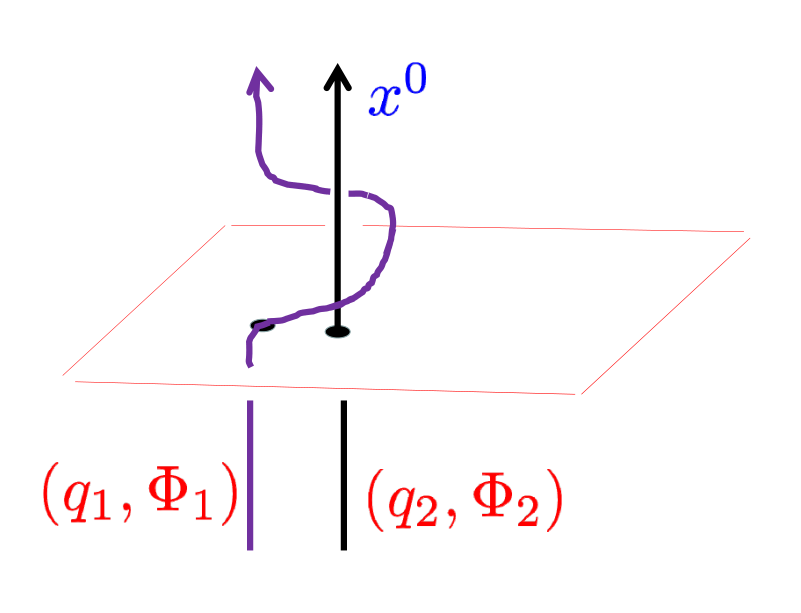
\includegraphics[width=0.6\textwidth]{figures/fig28.png}
  \caption{束缚态 $(q_1,\Phi_1)$ 极缓慢地沿逆时针方向绕过束缚态 $(q_2,\Phi_2)$。在计算波函数的相位变化时，只有路径的拓扑才有意义。不要把竖直方向与 $z$ 轴混淆：这里的竖直方向表示时间方向。（原文 Fig.~28，第 162 页）}
  \label{fig:28}
\end{figure}

让我们把粒子 $(q_1,\Phi_1)$ 极缓慢地绕过粒子 $(q_2,\Phi_2)$，如图~\ref{fig:28} 所示。应用公式 (??)，波函数获得相位 $\exp[\frac{\mathrm{i}}{\hbar c}(q_2\Phi_1)]$。注意这并不依赖轨迹的精确形状，只要求一个粒子绕着另一个转了一圈。与此同时，还有另一份相位变化，因为粒子 $(q_2,\Phi_1)$ 绕过了磁通 $\Phi_1$。事实上我们可以把图~\ref{fig:28} 形变成图~\ref{fig:29}。于是合起来，
% [Tutor Note: 原文此处和被引的「一般公式」都写作 "(??)"——作者源文件里这一交叉引用没有解析出来（应指后文 (10.2)–(10.4) 所在的那条一般公式，讲电荷绕磁通一周的 Aharonov-Bohm 相位）。这是原文自身的残缺，译文保留 "(??)" 以示未作补全]

\begin{figure}[htbp]
  \centering
  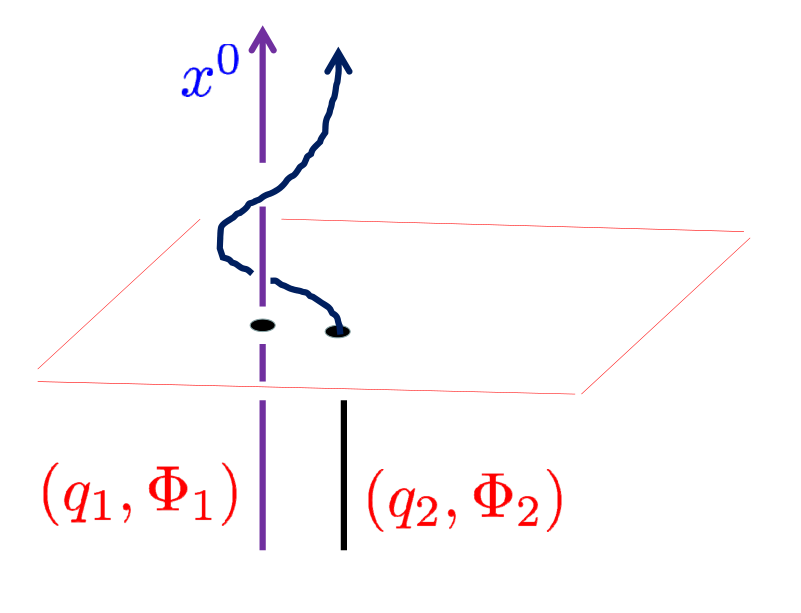
\includegraphics[width=0.6\textwidth]{figures/fig29.png}
  \caption{把 Figure~7 中的路径作拓扑等价的重新表述。由此可以清楚看出：束缚态 $(q_2,\Phi_2)$ 也沿逆时针方向绕 $(q_1,\Phi_1)$ 运动。（原文 Fig.~29，第 163 页）}
  \label{fig:29}
\end{figure}
% 原文疑似笔误：图注中的 "the path in Figure 7" 应为 "Figure 28"（本图的形变对象正是 Figure 28 中的路径）；照原文转写，未改

这对粒子的波函数改变为
\begin{equation}
  \exp\Big[\frac{\mathrm{i}}{\hbar}(q_2\Phi_1+q_2\Phi_2)\Big]
  \tag{10.1}
  \label{eq:10.1}
\end{equation}
% [Tutor Note: 原文 (10.1) 的第二项写作 $q_2\Phi_2$。按上下文（粒子 1 绕粒子 2 走、粒子 2 绕磁通 $\Phi_1$ 走，两份相位应分别为 $q_2\Phi_1$ 与 $q_1\Phi_2$），第二项似应为 $q_1\Phi_2$。此处照原式转写、未作改动，引用时请留意]

\begin{figure}[htbp]
  \centering
  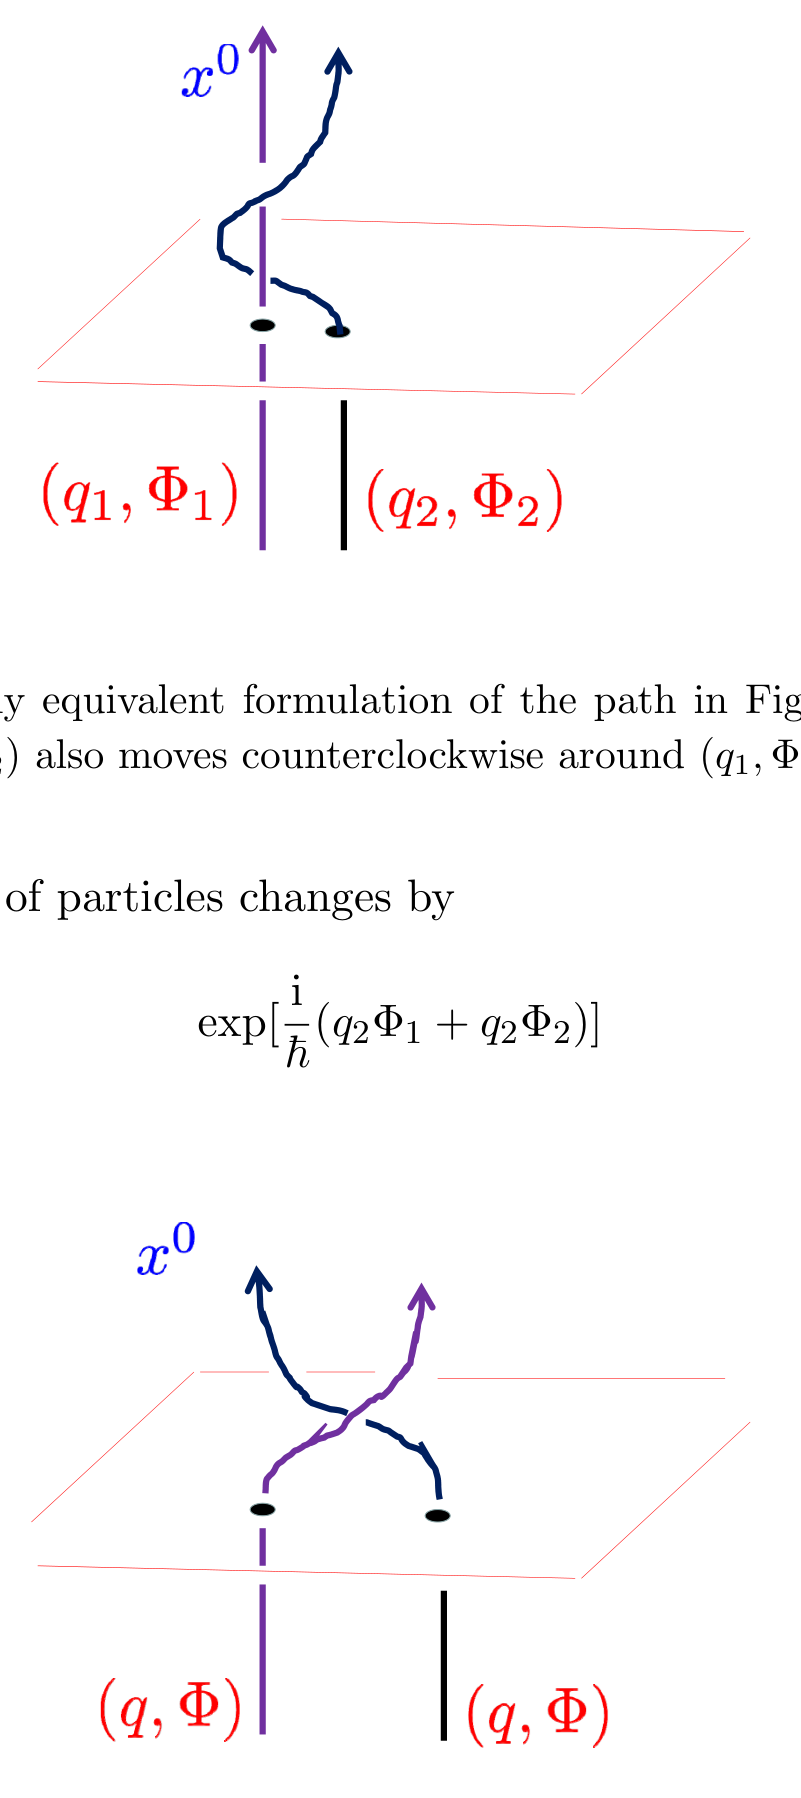
\includegraphics[width=0.6\textwidth]{figures/fig30.png}
  \caption{一对全同粒子 $(q,\Phi)$ 被交换。（原文 Fig.~30，第 163 页）}
  \label{fig:30}
\end{figure}

现在让我们考虑一对全同粒子，它们如图~\ref{fig:30} 所示被交换。净相位变化就是 $\exp[\mathrm{i}\frac{q\Phi}{\hbar}]$。但既然我们交换的是全同粒子，就可以把这个相位解释为统计相位。与 $3+1$ 维粒子的情形不同，在目前的情形下统计相位可以是\emph{任意}相位。这样的粒子称为任意子。\footnote{任意子的可能存在性由 Leinaas 与 Myrheim 于 1977 年指出。``anyon'' 一词则由 F. Wilczek 在 ``Quantum Mechanics of Fractional-Spin Particles''（Physical Review Letters \textbf{49} (14): 957-959）中提出。}

考察自旋与统计之间的关系是很有意思的。

现在我们把一般公式 (??) 用到 $d=2+1$ 维的角动量上。这里只有一个生成元 $J=J_{12}$。

在 $2+1$ 维中，螺线管贡献 $F_{ij}=\epsilon_{ij}\Phi\delta^2(x)$（这里 $i,j$ 取 $1$ 到 $2$，且 $\epsilon_{12}=+1$）。由 (??) 可知，位于 $\vec R$ 处的带电粒子贡献电场
\begin{equation}
  \vec E=2q\,\frac{\vec x-\vec R}{|\vec x-\vec R|^2}
  \tag{10.2}
  \label{eq:10.2}
\end{equation}
于是 $F_{0j}=-2q(x-R)^j/|\vec x-\vec R|^2$。因此动量密度为
\begin{equation}
  T_{0i}=F_{0k}F_{ik}=\frac{q\Phi}{2\pi}\epsilon_{ij}\frac{R_j}{R^2}\delta^{(2)}(\vec x)
  \tag{10.3}
  \label{eq:10.3}
\end{equation}
由于 $\delta$ 函数，积分很容易算出，我们得到
\begin{equation}
  J_{12}=\frac{q\Phi}{2\pi}\frac{\vec a\cdot\vec R}{\vec R\cdot\vec R}
  \tag{10.4}
  \label{eq:10.4}
\end{equation}
现在来检验自旋与统计的关系就很有趣了：
% [Tutor Note: (10.2)–(10.3) 中间那一步「$F_{0j}=-2q(x-R)^j/|\vec x-\vec R|^2$」里作者把矢量写成了标量 $(x-R)^j$（同页 (10.2) 用的是 $\vec x,\vec R$），转写时照原样保留。另外这一段用的显然是自然单位制（(10.3)、(10.4) 中没有 $c$），而 (10.1) 的相位里却出现了 $\hbar c$；核对量纲时请连同 $c$ 一起检查：作用是 $q\Phi/c$ 才与 $\hbar$ 同量纲]

\begin{figure}[htbp]
  \centering
  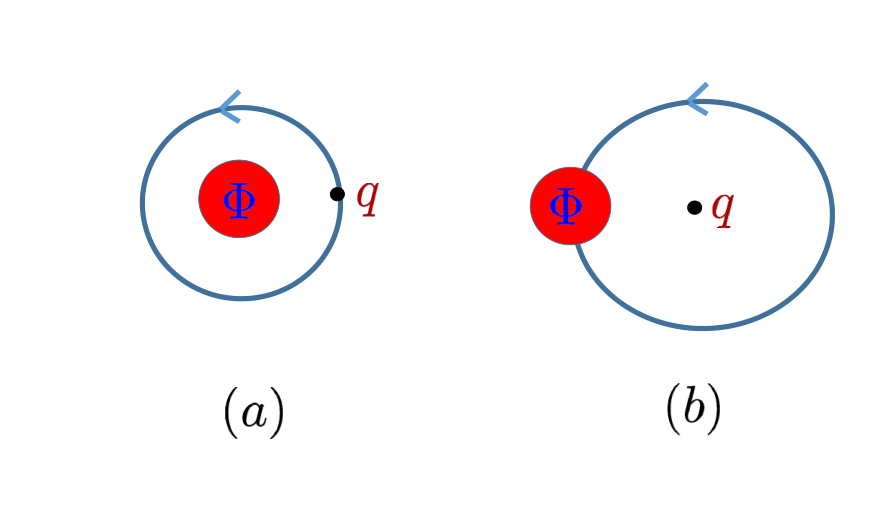
\includegraphics[width=0.8\textwidth]{figures/fig31.png}
  \caption{(a) 中电荷 $q$ 被缓慢地绕磁通子（fluxon）$\Phi$ 移动，波函数获得一个 Aharonov-Bohm 相位。(b) 中我们绕 $q$ 作一个 $2\pi$ 的旋转，电磁场的波函数也获得一个相位。这两个相位是相同的。（原文 Fig.~31，第 164 页）}
  \label{fig:31}
\end{figure}

\begin{enumerate}
  \item 若我们以逆时针方向缓慢地让粒子绕磁通转动，则波函数获得相位 $\exp[\mathrm{i}q\Phi/\hbar]$。
  \item 另一方面，若让磁通绕粒子转动，则波函数应当改变 $\exp[2\pi\mathrm{i}J/\hbar]$。在 \eqref{eq:10.4} 中取 $\vec a=\vec R$，我们得到同一个相位：
\end{enumerate}
\begin{equation}
  \exp[2\pi\mathrm{i}J/\hbar]=\exp[\mathrm{i}q\Phi/\hbar]
  \tag{10.5}
  \label{eq:10.5}
\end{equation}

\begin{remark}[自旋-统计定理]
证明自旋-统计定理时用到的重要性质，是存在到欧氏空间的解析延拓。
\end{remark}
% 原文此处是 "Remark Spin-statistics theorem: ..." 的格式；原文未给编号，译文用 remark 环境（编号由 LaTeX 自动给出）
{\small\itshape ［原文标记：Need to elaborate much more on that.（这一点需要再多讲很多。）］}
% [原文待办标记，原文 p.164；紧接在 remark 末句之后]

以下是一些关于任意子的更多材料来源：

\begin{enumerate}
  \item John Preskill 写了一些很好的讲义，其中讨论了与量子计算、量子信息理论的可能关联：\texttt{http://www.theory.caltech.edu/\textasciitilde presk}
  % 原文此行在 PDF 中被页面右边界截断（只印到 "presk"），译文照录截断后的字样
\end{enumerate}
